\chapter{Introduction}
\section{Lifetime and Degradation Science: Applicability to Renewable energy}

%%%%%%%%%%%%%%%%%%%%%%%%%%%%%%%%%%%%%%%%%%%
\subsection{Project Overview}

% Reinforcement Learning
Reinforcement Learning is a type of machine learning that allows you to create AI agents that learn from the environment by interacting with it. Just like how we learn to ride a bicycle, this kind of AI learns by trial and error. As seen in Figure 1, the brain represents the AI agent, which acts on the environment. After each action, the agent receives the feedback. The feedback consists of the reward and next state of the environment. The reward is usually defined by a human. If we use the analogy of the bicycle, we can define reward as the distance from the original starting point.

\begin{figure}[h]
\centering
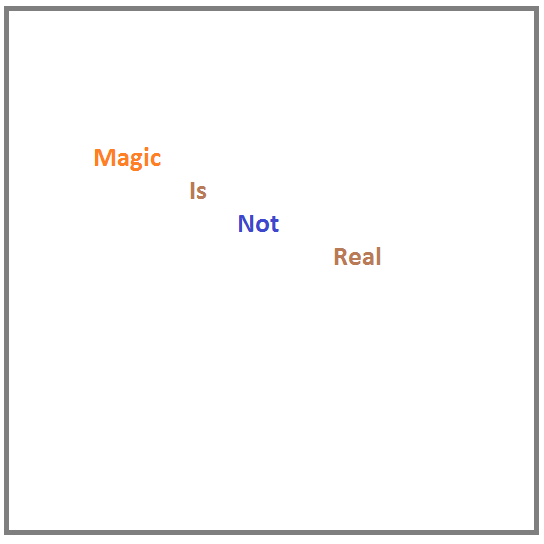
\includegraphics[width=0.5\textwidth]{figs/magic}
\caption{How an agent interacts with the environment.}
\end{figure}

% Deep Reinforcement Learning
Google's DeepMind published its famous paper Playing Atari with Deep Reinforcement Learning, in which they introduced a new algorithm called Deep Q Network (DQN for short) in 2013. It demonstrated how an AI agent can learn to play games by just observing the screen without any prior information about those games. The result turned out to be pretty impressive. This paper opened the era of what is called ?deep reinforcement learning?, a mix of deep learning and reinforcement learning.

%%%%%%%%%%%%%%%%%%%%%%%%%%%%%%%%%%%%%%%%%%%
\subsection{Problem Statement}

In this project, a deep reinforcement learning method, Deep Q Network, would be implemented and applied to play a Coast Racer game in OpenGym / Universe using TensorFlow.

% Q Learning
Q-learning, a model-free online off-policy algorithm, whose main strength is that it is able to compare the expected utility of the available actions without requiring a model of the environment. In Q-Learning Algorithm, there is a function called Q Function, which is used to approximate the reward based on a state. We call it Q(s,a), where Q is a function which calculates the expected future value from state s and action a. Similarly in Deep Q Network algorithm, we use a neural network to approximate the reward based on the state. We will discuss how this works in detail.


% Q function
\textbf{Target function:}

$Q^\pi : \mathcal{S} \times \mathcal{A} \to \mathbb{R}$, where $\mathcal{S}$ is the set of \emph{states} and $\mathcal{A}$ is the set of \emph{actions} (turn left, forward or turn right), and $\mathbb{R}$ represents the value of being in a state $s \in \mathcal{S}$, applying a action $a \in \mathcal{A}$, and following policy $\pi$ thereafter.

\textbf{Target function representation:}

Deep neural network.

Therefore, I seek to build a Q-learning agent trained via a deep convolutional neural network to approximate the optimal action-value function:

\begin{equation}
Q^*(s,a) = \max\limits_\pi Q^\pi(s,a), \forall s \in \mathcal{S}, a \in \mathcal{A}
\end{equation}

\noindent which is the maximum sum of rewards achievable by a behavior policy $\pi$.

%%%%%%%%%%%%%%%%%%%%%%%%%%%%%%%%%%%%%%%%%%%
\subsection{Metrics}

Since Q learning is recursively defined, we did not consider fitting errors such as RMSE to be good metrics for evaluation. Instead, given our ultimate our goal to make a good game AI, we evaluated gameplay directly in order to gauge performance. We evaluated the performance of our algorithms using two metrics: game length and game score. Game length is the number of moves the player makes before they reach a game over, and game score is the score based on the number of lines they clear. While the game score is ultimately more important, it can only be used to judge the performance of sufficiently advanced networks because there is a large initial barrier to overcome before the algorithm can score with any degree of consistency. Thus, game length, which was typically correlated with game score, is a good metric for showing intermediate performance since an algorithm can incrementally learn to survive longer.
      
%%%%%%%%%%%%%%%%%%%%%%%%%%%%%%%%%%%%%%%%%%%%%%%%%%%%%%%%%%%%%%%%%%%%%%%%%%%%%%%%%%%%%%%%%%%%%%%%%%%%



%\bibliographystyle{plainnat}
%\markright{\textit{Bibliography}}
%\renewcommand{\chaptername}{}
%x\bibliography{KL-Thesis}

\vfill

